\documentclass[11pt,titlepage]{article}
\usepackage{geometry}
\geometry{
	a4paper,
	left=20mm,
	right=20mm,
	top=15mm,
	bottom=15mm,
}
\usepackage{tikz}
\usetikzlibrary{arrows,backgrounds}
\usepgflibrary{shapes.multipart}
\usepackage{graphicx}
\usepackage{mathtools}
\usepackage{inputenc}
\usepackage{amssymb}
\usepackage{wrapfig}
\usepackage{seqsplit}
\usepackage{float}
\usepackage[font=scriptsize]{caption} 
\linespread{1.0}
\usepackage{caption}
\renewcommand{\figurename}{Fig.}
\usepackage{subcaption}
\usepackage[title]{appendix}
\usepackage{enumitem}
\usepackage{listings}
\usepackage{xcolor}
\definecolor{codegreen}{rgb}{0,0.6,0}
\definecolor{codegray}{rgb}{0.5,0.5,0.5}
\definecolor{codepurple}{rgb}{0.58,0,0.82}
\definecolor{backcolour}{rgb}{0.95,0.95,0.92}

\lstdefinestyle{mystyle}{
	backgroundcolor=\color{backcolour},   
	commentstyle=\color{codegreen},
	keywordstyle=\color{magenta},
	numberstyle=\tiny\color{codegray},
	stringstyle=\color{codepurple},
	basicstyle=\ttfamily\tiny,
	breakatwhitespace=false,         
	breaklines=true,                 
	captionpos=b,                    
	keepspaces=true,                 
	numbers=left,                    
	numbersep=5pt,                  
	showspaces=false,                
	showstringspaces=false,
	showtabs=false,                  
	tabsize=2
}

\lstset{style=mystyle}
\setlength{\columnsep}{5pt}

%opening
\title{EECE6036: Intelligent Systems\\Homework \# 5}
\author{Zuguang Liu (M10291593)}



\begin{document}

\maketitle

\section{Self-Organized Feature Map (SOFM)}





\subsection{Problem Statement}

In this problem, a SOFM is implemented and trained on the MNIST dataset. The map consists of 12 $\times$ 12 neurons, each of which is a 784-long vector that forms the input layer. 









\subsection{System Description}
Using the same stratified sampling policy the previous Homework used, the preprocessing section splits the total 5,000 data points into 4,000 for training and 1,000 for testing, where there are 400 and 100 images for each model respectively. This balanced partition controls the training by letting the model adjust to equal amount of data over all classes. 

\textbf{Weights are initialized based on the first six principal components of the training data} from Singular Value Decomposition process. The six vectors are linearly combined in a random fashion to form the initial weights of 144 neurons.

\textbf{The training of the model is a two-phase process}, where each phase is also dynamic with gradually decreasing learning rate (\ref{eqn:eta}), and gradually centralized neighborhood function (\ref{eqn:sigma}, $\sigma$ is the standard deviation in the Gaussian function). Weights are adjusted per data point, repeated for multiple epochs (as in $t$). Specifically,

\begin{enumerate}
	\item In self-organizing phase, $t = 1,000, \eta_0 = 0.1, \tau_L=1,000, \sigma_0 = 8.5, \tau_N = 467$. These values are set so that the neighborhood function starts from covering most of the map, to only cover the winning unit at the end.
	
	\item In convergence phase, the training slowly adjusts weights that only belong to the winning unit for 500 epochs. This is done by setting $t = 500, \eta_0 = 0.01, \tau_L \approx \infty, \sigma_0 \approx 0, \tau_N \approx \infty$.
\end{enumerate}

\begin{equation}
	\eta (t) = \eta_0 \exp(-t/\tau_L)
	\label{eqn:eta}
\end{equation} 

\begin{equation}
	\sigma(t) = \sigma_0 \exp (-t / \tau_N)
	\label{eqn:sigma}
\end{equation}

After training, the resulting model is analyzed using the test dataset. 












\subsection{Results}
Fig. \ref{fig:heatmap} shows heat maps for each class, where in each plot, the winning rate of the 12 $\times$ 12 neurons are presented by a greyscale pixel (dark pixels means low winning rate), and the pixels are mapped in the same configuration as the neurons. 

The weights of the neurons at the end of the training are demonstrated in Fig. \ref{fig:feature}, with the same mapping fashion as designed. 

\begin{figure}[H]
	\centering
	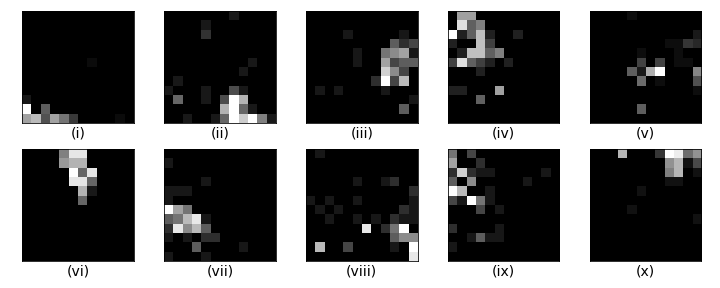
\includegraphics[width=\linewidth]{img/h5p1_heat}
	\caption{Heat map of the neurons separated by classes. The plot label uses roman letters that also represent the class of the images, for example, (i) uses images of digit `1'. Digit `0' is shown in (x).}
	\label{fig:heatmap}
\end{figure}

\begin{figure}[H]
	\centering
	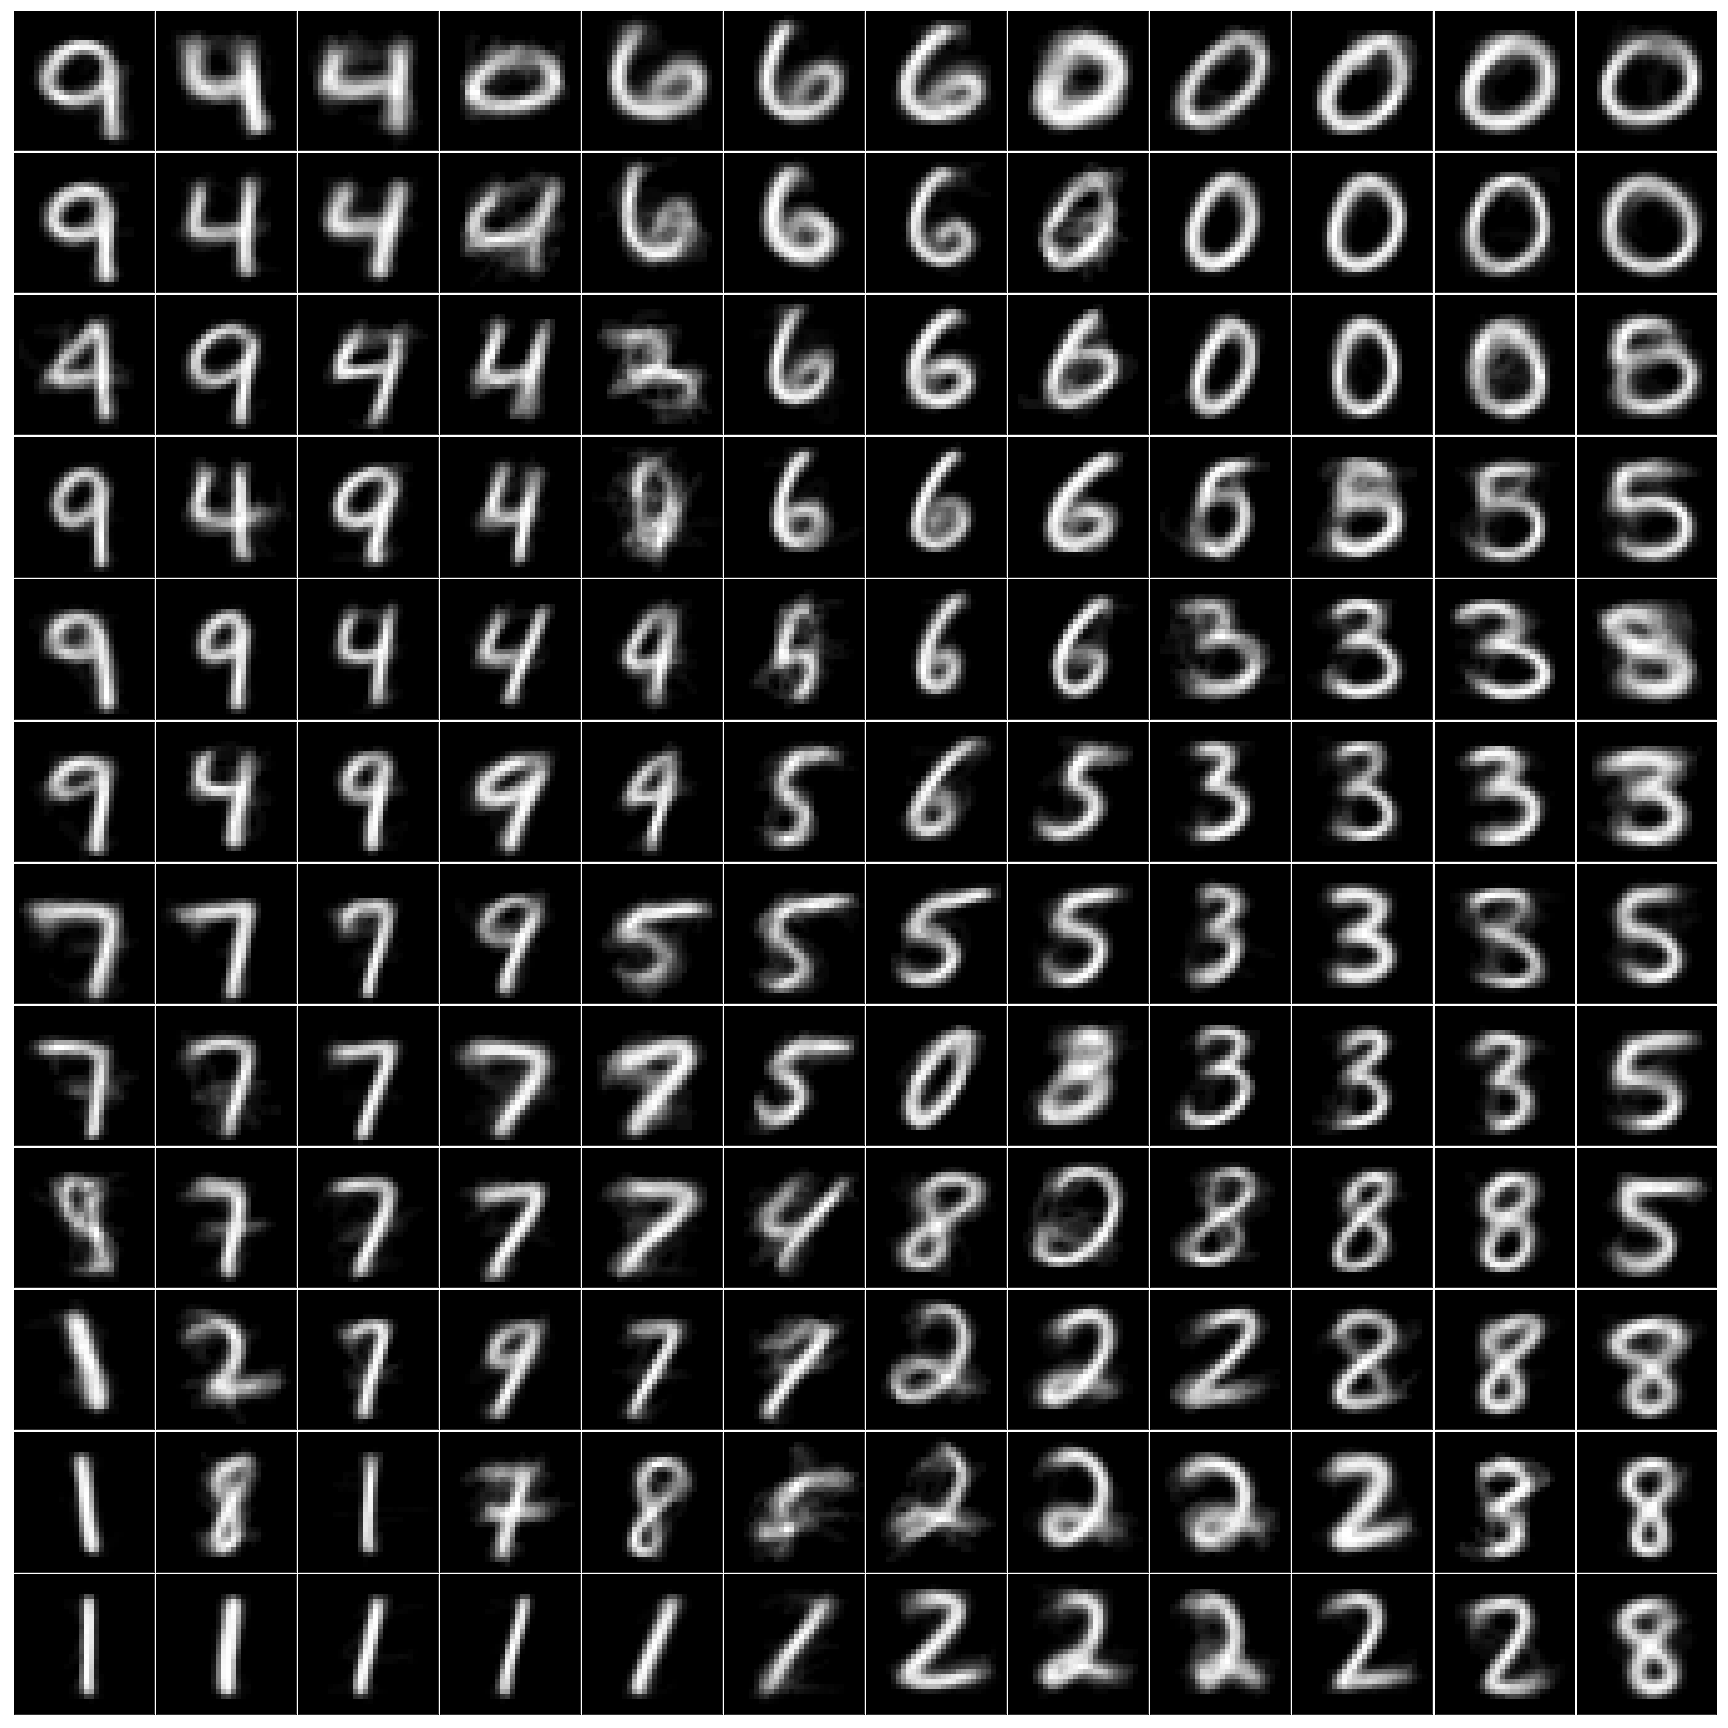
\includegraphics[width=\linewidth]{img/h5p1_feature}
	\caption{Feature map of the neurons in a 12 $\times$ 12 configuration}
	\label{fig:feature}
\end{figure}










\subsection{Analysis of Results}
The feature map in Fig. \ref{fig:feature} shows great resemblance with the looks of the original data, making the resulting model successful and explainable. The map does not only demonstrates the evolution on how the model interprets the image data, but also groups similar image patterns together. For example, in the lower left corner of the map, there are a few drawings of digit `1' with small levels of variations. Then going from this corner to the lower right corner, images that look like `2' and `8' are shown, where the visual complexity of the image pattern increases gradually.

With the grouping pattern found in the feature map, it is not surprising to find that spatially close neurons fire together in choosing the winner in heat maps, and that winning neurons all have feature maps that look like corresponding digits as well. The upper right corner of Fig. \ref{fig:feature} is populated with images that look like `0', so accordingly, neurons at the upper right corner mostly win when the model is presented with test data of class `0' in Fig. \ref{fig:heatmap} (x).  

\newpage






\section{Classifiers Based on SOFM}
\subsection{Problem Statement}

Using the trained SOFM as a hidden layer, a classifier can be constructed with an additional output layer that infers the class of images. After training, the performance of the two networks shall be compared and contrasted together with the classifier from Homework \#3 whose hidden layer is initialized randomly, and the two classifiers from Homework \# 4 whose hidden layer comes from autoencoders.

To tell apart the models, the report uses \textbf{SOFM classifier} to address this new model, and calls the two autoencoder-based network \textbf{denoising classifier} and \textbf{reconstructing classifier}, as the original autoencoders are to reduce noise or reconstruct the image. The last one from Homework \#3 whose hidden layer is initialized randomly shall be called \textbf{BP classifier} as the gradient back-propagates to the first layer to adjust its weights, while only the output layer applies the weight change for the other models.







\subsection{System Description}
To control the training settings, \textbf{all four classifiers are trained with exactly the same data, algorithm and hyper-parameters}. Since the previous Homework used 128 neurons instead of 144, the relevant models are adjusted to 144 neurons and trained again. 

Similar to the previous Homework, the SOFM connects to an output layer of 10 neurons, each of which represents the possibility of the image belonging to a class. To implement forward feeding from the SOFM to the output layer, ``winner-take-all'' strategy is used, so only the winner outputs 1 and the rest is 0. Finally, to decide on the label, neurons with the highest output are selected. 

The training proceeds similarly to the previous Homework. Back propagation with momentum ($\eta = 0.1, \alpha = 0.8$) is used, iterated over all data points and repeated for 500 epochs. Only the weights of the output layer is adjusted. Threshold of 0.25 and 0.75 are used for consistent hyperparameter set though not practically applicable. Regularization methods include weight decay ($\lambda = 10^{-5}$) and validation-based early stopping (50 epochs patience). 


After training, the test dataset is presented to all mentioned classifying networks.








\subsection{Results}
Time series of on-line training loss on SOFM classifer is presented in Fig. \ref{fig:classifier_train}. Fig. \ref{fig:cm} shows the confusion matrices of the four classifiers on train data and test data.

\begin{figure}[H]
	\centering
	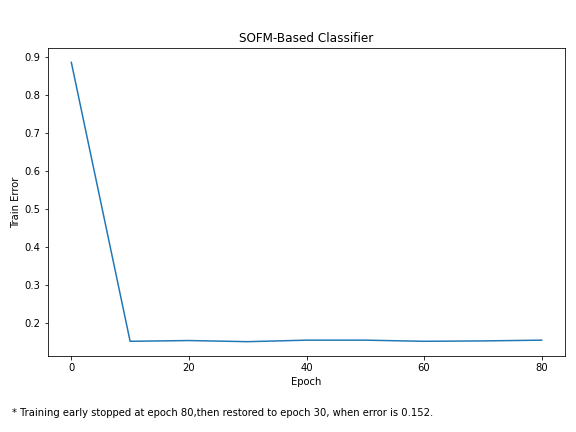
\includegraphics[width=0.7\linewidth]{img/h5p2_train}
	\caption{Error vs epochs during training of SOFM classifier}
	\label{fig:classifier_train}
\end{figure}

\begin{figure}[H]
	\centering
	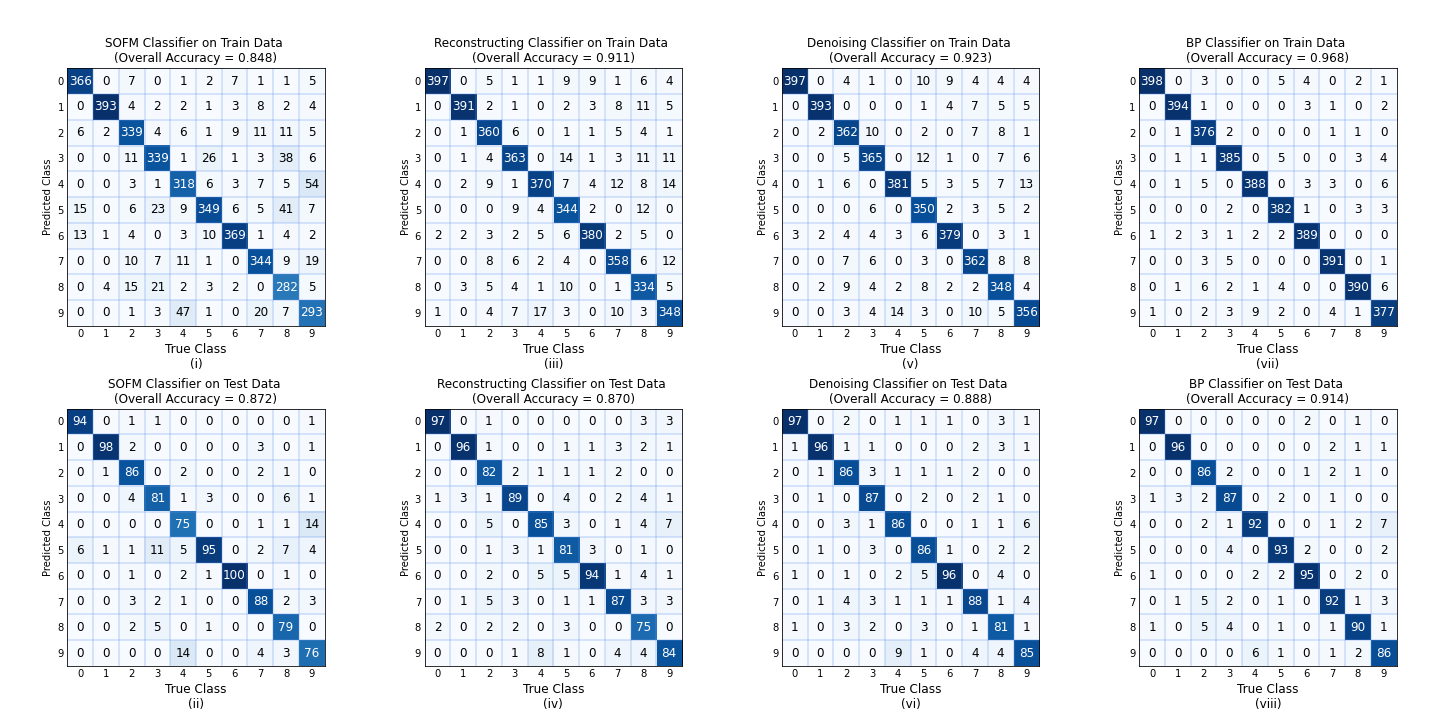
\includegraphics[width=\linewidth]{img/h5p2_cm}
	\caption{Performance of four classifier implemented so far}
	\label{fig:cm}
\end{figure}

\subsection{Analysis of Results}
The accuracy of the SOFM classifer is slightly higher than that of the reconstructing classifier, making it an acceptable candidate for the classification problem. It is also unexpected to see the accuracy on the test dataset is higher than that on the train dataset, which is not the case for any other models, suggesting that the SOFM classifier is more robust in terms of preventing overfitting. Moreover, since the features of the SOFM look visually close to the original images (Fig. \ref{fig:feature}), it is easy to identify the source of error and adjust accordingly. For example, in Fig. \ref{fig:cm} (ii), there are 14 images of digit `4' classified as `9' and vice versa, which is explainable by the fact that feature maps that look like `4` and `9' are not distinctly separated in Fig. \ref{fig:feature}.

The four models, including SOFM classifier, reconstructing classifier, denoising classifier, and BP classifier, took 47 min, 15 min, 14 min, and 12 min collectively to train. More optimization can be done admittedly, but it is a fact that a simple two-layer fully-connected neural network has the best accuracy with the least computational effort. However, though having the longest training time and mediocre accuracy, SOFM classifer has undeniably high robustness and explainability, and therefore some potential to assist on highly complex deep networks.


\newpage
\begin{appendices}
\section{Python Code: preprocess.py}
\lstinputlisting[language=Python]{code/preprocess.py}

\newpage
\section{Python Code: nn.py}
\lstinputlisting[language=Python]{code/nn.py}

\newpage
\section{Python Code: sofm.py}
\lstinputlisting[language=Python]{code/sofm.py}

\newpage
\section{Python Code: h5p1\_train.py}
\lstinputlisting[language=Python]{code/h4p1_train.py}

\newpage
\section{Python Code: h5p1\_test.py}
\lstinputlisting[language=Python]{code/h4p1_test.py}

\newpage
\section{Python Code: h5p2\_train.py}
\lstinputlisting[language=Python]{code/h4p2_train.py}

\newpage
\section{Python Code: h5p2\_test.py}
\lstinputlisting[language=Python]{code/h4p2_test.py}

\end{appendices}

\end{document}